\def\sectiontitle{WIPP plugins for AI models reuse}

\section{\sectiontitle}

%%%%%%%%%%%%%%%%%%%%%%%%%%%%%%%%%%%%%%%%%%%%%%%%%%%%%%%%%%%%%%%%%%%%%%%%%%%%%%%%
\def\slidetitle{Public AI repositories}

\subsection{\slidetitle}
\begin{frame}
  \frametitle{\sectiontitle}
  \framesubtitle{\slidetitle}

  Many public AI models on lots of public AI repositories

  \begin{center}
    \begin{table}
      \begin{tabular}{|c|c|c|}
       \hline
       \rowcolor{tableFirstRowColor} AI repositories & Image classification models & Segmentation + MG* models \\ [0.5ex]
       \hline
       \cellcolor{tableFirstColColor} Hugging Face & 15,593 & 1,160 + 176 \\
       \hline
       \cellcolor{tableFirstColColor} BioImage.IO & 1 & 4 + 32 \\
       \hline
       \cellcolor{tableFirstColColor} Cellpose & $\times$ & 21 \\
       \hline
       \cellcolor{tableFirstColColor} SAM2 & $\times$ & 8 \\
       \hline
       \cellcolor{tableFirstColColor} PyTorch Hub & 20 & 5 \\
       \hline
      \end{tabular}
      \caption{Number of models per repository}
    \end{table}
  \end{center}

  * MG: Mask Generation

\end{frame}

%%%%%%%%%%%%%%%%%%%%%%%%%%%%%%%%%%%%%%%%%%%%%%%%%%%%%%%%%%%%%%%%%%%%%%%%%%%%%%%%
\def\slidetitle{Unlock these repositories}

\subsection{\slidetitle}
\begin{frame}
  \frametitle{\sectiontitle}
  \framesubtitle{\slidetitle}

  \begin{minipage}[h!]{0.53\textwidth}
    Goal: Access external AI models in WIPP

    \bigskip

    Work:

    Plugins for Hugging Face, BioImage.IO, Cellpose and more public repositories

    \bigskip

    Question:

    How to assess the relevance of results?

  \end{minipage}\hfill
  \begin{minipage}[h!]{0.46\textwidth}
    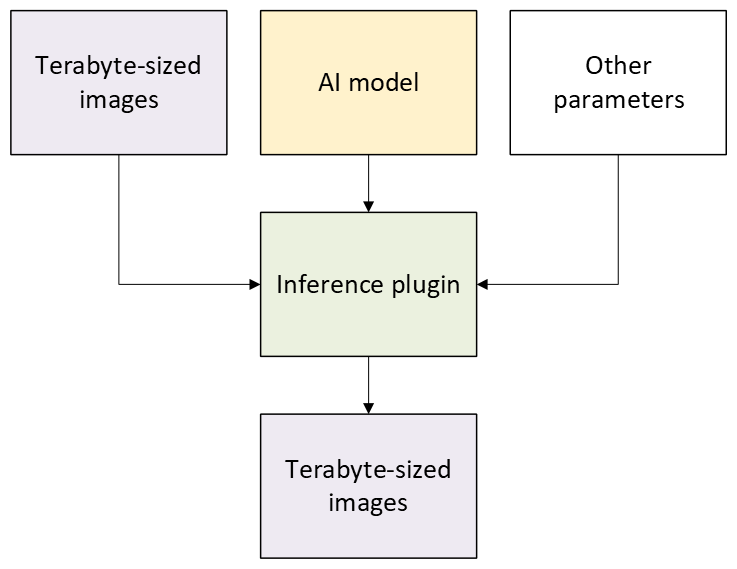
\includegraphics[scale=0.55]{./img/2_ai-plugins/inference.png}
  \end{minipage}
\end{frame}

%%%%%%%%%%%%%%%%%%%%%%%%%%%%%%%%%%%%%%%%%%%%%%%%%%%%%%%%%%%%%%%%%%%%%%%%%%%%%%%%
\def\slidetitle{Evaluate results}

\subsection{\slidetitle}
\begin{frame}
  \frametitle{\sectiontitle}
  \framesubtitle{\slidetitle}

  \begin{minipage}[h!]{0.65\textwidth}
    Goal: Mesure accuracy of external AI results

    \bigskip

    Work:

    Plugin to compute the Dice-Sørensen coefficient*

    \bigskip
    \bigskip

    *Statistic used to gauge the similarity of two samples
  \end{minipage}\hfill
  \begin{minipage}[h!]{0.35\textwidth}
    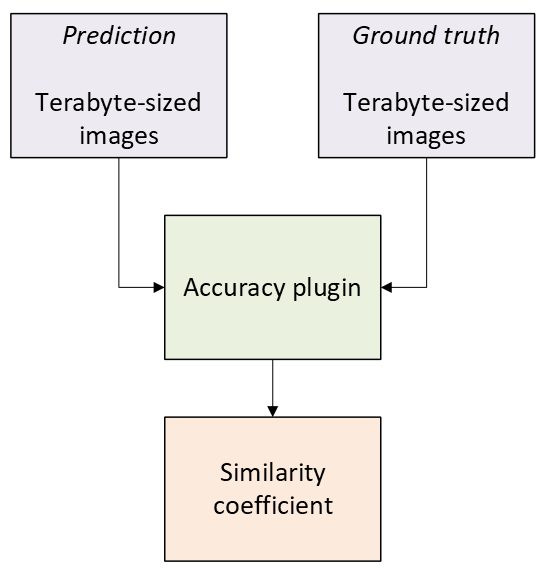
\includegraphics[scale=0.55]{./img/2_ai-plugins/accuracy.png}
  \end{minipage}
\end{frame}
